\documentclass{standalone}
\usepackage{tikz}
\usetikzlibrary{angles}

\begin{document}
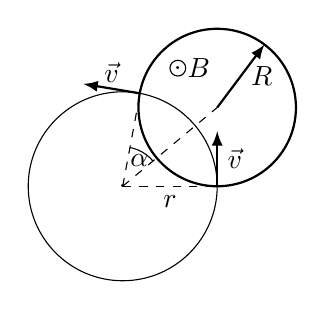
\begin{tikzpicture}
    \coordinate (A) at (-0.98, 0.18);
    \coordinate (B) at (-1.2,-1);
    \coordinate (C) at (0,-1);
    \coordinate (O) at (0,0);
	\draw [thick] (0,0) circle (1);
	\draw [] (-0.5,0.5) circle (0.1) node [] {.} node [right] {$B$};
	\draw [] (-1.2,-1) node [] {.};
	\draw [dashed] (-1.2, -1) -- (0, -1) node [midway, below] {$r$};
	\draw [dashed] (-1.2, -1) -- (-0.98, 0.18);
	\draw [] (-1.2, -1) circle (1.2);
	\draw [dashed] (B)--(O);
	\draw [arrows={-latex}, thick] (0, 0) -- (0.6, 0.8) node [midway, right]  {$R$};
	\draw [arrows={-latex}, thick] (0, -1) -- (0, -0.3) node [midway, right]  {$\vec{v}$};
	\draw [arrows={-latex}, thick] (-0.98, 0.18) -- (-1.7, 0.3) node [midway, below=-13pt]  {$\vec{v}$};
	\pic [draw, -, angle eccentricity=1.6] {angle = O--B--A};
	\node [right=6pt, below=-15pt] at (B) {$\alpha$};
\end{tikzpicture}
\end{document}